%% UniMemory - Final Year Project Research Paper
%% IEEE conference two-column format.
%% Compile: pdflatex main.tex ; bibtex main ; pdflatex main ; pdflatex main
%%
\documentclass[conference]{IEEEtran}
\IEEEoverridecommandlockouts

\usepackage{cite}
\usepackage{amsmath,amssymb,amsfonts}
\usepackage{graphicx}
\usepackage{booktabs}
\usepackage{array}
\usepackage{listings}
\usepackage{xcolor}
\usepackage{url}
\usepackage{tikz}
\usetikzlibrary{arrows.meta,positioning}
\usepackage[hidelinks]{hyperref}

% ---- TikZ styles -----------------------------------------------------------
\tikzset{
  box/.style={draw,rounded corners=2pt,align=center,font=\scriptsize,
    minimum height=0.8cm,minimum width=2.0cm,inner sep=2pt,fill=white},
  wide/.style={box,minimum width=8.2cm},
  arr/.style={-{Stealth[length=4pt]},thick},
  opt/.style={dashed}
}

\renewcommand{\ttdefault}{cmtt} % use CM typewriter (avoids missing Courier TFM)
\lstset{basicstyle=\ttfamily\footnotesize,breaklines=true,
        frame=single,columns=fullflexible,aboveskip=8pt}

\begin{document}

\title{UniMemory: Design, Implementation and Evaluation of a\\
Long-Term Memory Infrastructure for AI Applications}

\author{\IEEEauthorblockN{Shreyas Gurav, Raj Tripathi, Soumya Patil, and Parth Gandhi}
\IEEEauthorblockA{Group 2 (roll nos.\ 16014223078, 16014223062, 16014223084, 16014223059)\\
Department of Information Technology, B.Tech.\ AI \& Data Science\\
K~J~Somaiya School of Engineering, Somaiya Vidyavihar University, Mumbai, India\\
Guide: Mr.\ Sunil Shelke \quad External guide: Mr.\ Kunal Parekh, CPO, Osmos\\
Code: \url{https://github.com/shreyasgurav/UniMemory}}}

\maketitle

% ============================================================ ABSTRACT
\begin{abstract}
Large language model (LLM) assistants are largely stateless: each session
starts without knowledge of prior interactions, forcing users to re-establish
context and preventing personalization. This paper presents UniMemory, a
long-term memory infrastructure that captures raw interactions from AI tools,
extracts durable atomic memories, deduplicates and embeds them, links them into
a semantic graph, and serves them back to any application through a REST API,
language SDKs, a Model Context Protocol (MCP) server, and a browser extension.
We describe the ingestion pipeline and a hybrid retrieval mechanism that
re-ranks a vector-search candidate pool using lexical overlap, tag matching and
sector-aware similarity. We built a reproducible evaluation harness over a
synthetic persona corpus. Preliminary results on a development set (6 queries,
12 exact and paraphrased instances, 31 extracted memories) show that hybrid
re-ranking raises hit@1 from 6/12 (cosine only) to 9/12, that extracted memories
match raw-chat retrieval (hit@1 5/6 for both) while injecting fewer context
tokens (55 vs.\ 87 per query), and, as a sanity check, that an automated keyword
rubric scores answers 0.00 without memory and 1.67 with it (maximum 2). These
pilot results are indicative only; the final held-out evaluation, latency and
deduplication measurements are in progress and are not reported here.
\end{abstract}

\begin{IEEEkeywords}
long-term memory, AI agents, retrieval-augmented generation, Model Context
Protocol, semantic search, vector databases, personalization
\end{IEEEkeywords}

% ============================================================ 1 INTRODUCTION
\section{Introduction}
\subsection{Background}
Modern AI assistants are predominantly \emph{stateless}. A conversation held in
one tool on one day is invisible to the same tool the next day, and entirely
invisible to a different tool. As users increasingly spread work across multiple
assistants (chat interfaces, IDE copilots, browser agents), the absence of a
shared, persistent memory becomes a first-order limitation: users repeat the
same context, and assistants cannot personalize beyond the current window.

\subsection{Problem Statement}
Consider a user who, on Day~1, tells an assistant that they are vegetarian and
allergic to peanuts. On Day~2, in a fresh session---or in a different
tool---the same user asks for a recipe and receives a suggestion containing
peanuts. The information existed; it simply was not retained or shared. The
core problem is the lack of a reusable memory layer that (a) decides what is
worth remembering, (b) stores it durably, (c) retrieves it by meaning, and
(d) is accessible from any application.

\subsection{Objectives and Scope}
This work designs, implements and evaluates UniMemory, a long-term memory
infrastructure for AI applications. The developer-facing layer (REST API, SDKs,
API-key management, developer console) was built in the first phase; the
consumer-facing layer (consumer dashboard with memory-graph visualization,
browser extension, and MCP integration for AI coding tools) was built in the
second phase. This paper documents both and evaluates the end-to-end system.

\subsection{Contributions}
\begin{enumerate}
\item A deployed, end-to-end memory infrastructure spanning ingestion,
extraction, deduplication, embedding, semantic-graph construction and
retrieval, exposed through REST, SDKs, MCP and a browser extension.
\item An evaluation of a hybrid re-ranking scheme over vector-search candidates
(boosted similarity, lexical overlap, tag match, sector weighting), adapted from
OpenMemory~\cite{openmemory}, against lexical-only and pure-cosine scoring on the
same candidate pool.
\item An empirical evaluation on a reproducible synthetic corpus measuring
memory-on vs.\ memory-off quality, structured vs.\ raw-chat retrieval, the
scoring ablation, and operational latency/deduplication cost.
\end{enumerate}

\subsection{Paper Organization}
Section~\ref{sec:related} surveys related memory systems. Section~\ref{sec:design}
describes the architecture, pipeline, data model and retrieval mechanism.
Section~\ref{sec:impl} details the implementation and integrations.
Section~\ref{sec:method} defines the evaluation methodology and
Section~\ref{sec:results} reports results. Section~\ref{sec:casestudy} presents
a cross-tool case study. Sections~\ref{sec:discussion}--\ref{sec:conclusion}
discuss limitations and conclude.

% ============================================================ 2 RELATED WORK
\section{Related Work}\label{sec:related}
\subsection{Memory Systems for LLM Agents}
Recent systems add persistent memory to LLM agents. Mem0~\cite{mem0} extracts
and consolidates salient memories from conversations and evaluates a
production-oriented pipeline, including a graph-based variant. Zep~\cite{zep}
builds a temporal knowledge graph over conversational and business data.
A-MEM~\cite{amem} organizes memories as interlinked atomic notes that evolve
over time. MemGPT~\cite{memgpt} manages the LLM context window like virtual
memory, paging information between tiers, and MemoryBank~\cite{memorybank}
adds long-term memory with forgetting to a conversational companion.
OpenMemory~\cite{openmemory} (CaviraOSS, since renamed LongMemory) is the
closest open-source design to ours: in its earlier releases it classifies
memories into five cognitive sectors (semantic, episodic, procedural, emotional,
reflective) and links them with a waypoint graph and coactivation reinforcement.
LongMem~\cite{longmem} instead augments the model itself with a decoupled
long-term memory module, and PAM~\cite{pam} proposes a protocol for
cryptographically verified transfer of agent memory across heterogeneous agents,
addressing portability at the protocol level. Surveys~\cite{surveyA,surveyB,%
surveyC,surveyD} catalogue memory mechanisms, operations and open problems.

\subsection{Portability and Protocols}
The Model Context Protocol (MCP)~\cite{mcp} standardizes how external tools and
data sources are exposed to AI clients. UniMemory implements an MCP server so
memory becomes a tool available to MCP-capable assistants (e.g.\ Cursor, Claude
Desktop, Windsurf).

\subsection{Retrieval-Augmented Generation}
Retrieval-augmented generation (RAG)~\cite{rag} conditions generation on
retrieved text. UniMemory can be seen as a \emph{persistent, cross-application}
RAG substrate whose retrieval units are extracted atomic memories rather than raw
document chunks; Section~\ref{sec:results} compares the two on a small corpus.

\subsection{Gap Analysis}
Table~\ref{tab:related} summarizes algorithmic features as described in each
cited paper; it is not a benchmark. We do not claim to invent persistent memory
or to outperform these systems. Mem0, for instance, also offers SDKs and MCP
integration according to its public documentation. Our contribution is a
student-built, deployed, end-to-end stack (ingestion, retrieval, SDKs, MCP,
browser extension, two dashboards) together with a small, reproducible
evaluation of extracted-memory retrieval and a scoring ablation.

\begin{table}[t]
\caption{Algorithmic features as described in each system's source
(-- = not described there).}
\label{tab:related}
\centering
\footnotesize
\begin{tabular}{@{}lcccc@{}}
\toprule
System & LLM extraction & Vector search & Graph links & Temporal \\
\midrule
Mem0~\cite{mem0}       & \checkmark & \checkmark & \checkmark & -- \\
Zep~\cite{zep}         & \checkmark & \checkmark & \checkmark & \checkmark \\
A-MEM~\cite{amem}      & \checkmark & \checkmark & \checkmark & -- \\
MemGPT~\cite{memgpt}   & \checkmark & \checkmark & -- & -- \\
OpenMemory~\cite{openmemory} & -- & \checkmark & \checkmark & \checkmark \\
UniMemory              & \checkmark & \checkmark & \checkmark$^{a}$ & recency$^{b}$ \\
\bottomrule
\end{tabular}\\[2pt]
{\scriptsize $^{a}$Waypoint edges are stored and used for visualization; graph
expansion at retrieval time rarely triggers. $^{b}$Recency score only, not
exercised in our evaluation.}
\end{table}

% ============================================================ 3 SYSTEM DESIGN
\section{System Design and Architecture}\label{sec:design}
\subsection{Design Requirements}
Functional: ingest raw text/chat/documents; extract durable memories; semantic
search; multi-tenant isolation (owner, API key, end-user, project); provenance
from memory to source. Non-functional: stable public contract for SDKs;
heavy processing off the request's critical path; horizontal deployability.

\subsection{High-Level Architecture}
Figure~\ref{fig:arch} shows the layers: input sources (browser extension, API
clients, dashboards, MCP clients) feed a FastAPI service; a processing pipeline
transforms raw content into memories; a storage layer (PostgreSQL + pgvector)
holds raw sources, distilled memories and a memory graph; a retrieval engine
serves applications.

\begin{figure}[t]
\centering
\resizebox{\columnwidth}{!}{%
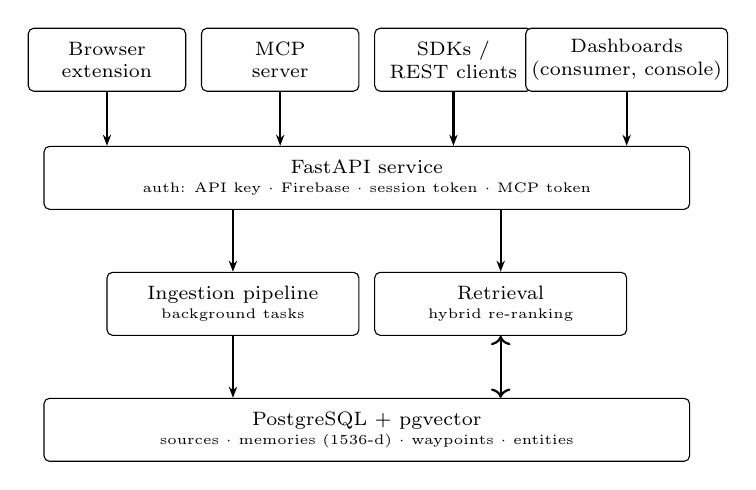
\begin{tikzpicture}
\node[box] (ext) at (0,0) {Browser\\extension};
\node[box] (mcp) at (2.2,0) {MCP\\server};
\node[box] (sdk) at (4.4,0) {SDKs /\\REST clients};
\node[box] (dash) at (6.6,0) {Dashboards\\(consumer, console)};
\node[wide] (api) at (3.3,-1.5) {FastAPI service\\[-1pt]{\tiny auth: API key $\cdot$ Firebase $\cdot$ session token $\cdot$ MCP token}};
\node[box,minimum width=3.2cm] (pipe) at (1.6,-3.1) {Ingestion pipeline\\[-1pt]{\tiny background tasks}};
\node[box,minimum width=3.2cm] (ret) at (5.0,-3.1) {Retrieval\\[-1pt]{\tiny hybrid re-ranking}};
\node[wide] (db) at (3.3,-4.7) {PostgreSQL + pgvector\\[-1pt]{\tiny sources $\cdot$ memories (1536-d) $\cdot$ waypoints $\cdot$ entities}};
\foreach \n in {ext,mcp,sdk,dash} \draw[arr] (\n.south) -- (\n.south |- api.north);
\draw[arr] (pipe.north |- api.south) -- (pipe.north);
\draw[arr] (ret.north |- api.south) -- (ret.north);
\draw[arr] (pipe.south) -- (pipe.south |- db.north);
\draw[arr,<->] (ret.south) -- (ret.south |- db.north);
\end{tikzpicture}}
\caption{High-level architecture. Clients share one backend and one store.}
\label{fig:arch}
\end{figure}

\subsection{Ingestion and Processing Pipeline}
On ingestion the raw source is persisted immediately and heavy work runs in the
background (Figure~\ref{fig:pipeline}):
\begin{enumerate}
\item \textbf{Worthiness gate.} A lightweight LLM check decides whether the
content is worth remembering; on timeout it \emph{fails open} (defaults to
worth-remembering).
\item \textbf{Summarization and extraction} run in parallel: a source summary
is generated, and up to 15 atomic memories are extracted per request.
\item \textbf{Deduplication.} Each candidate memory is reduced to a 64-bit
SimHash; if its Hamming distance to an existing memory is $\le 3$ it is treated
as a duplicate and instead \emph{reinforces} the existing memory's salience.
\item \textbf{Embedding.} Unique memories are embedded in parallel with
\texttt{text-embedding-3-small} (1536 dimensions).
\item \textbf{Storage and provenance.} Memories are written and linked N:N to
their source.
\item \textbf{Graph construction.} A background job creates
\emph{waypoint} edges to semantically similar memories (cosine $\ge 0.50$,
capped at five edges per memory).
\end{enumerate}

\begin{figure}[t]
\centering
\resizebox{\columnwidth}{!}{%
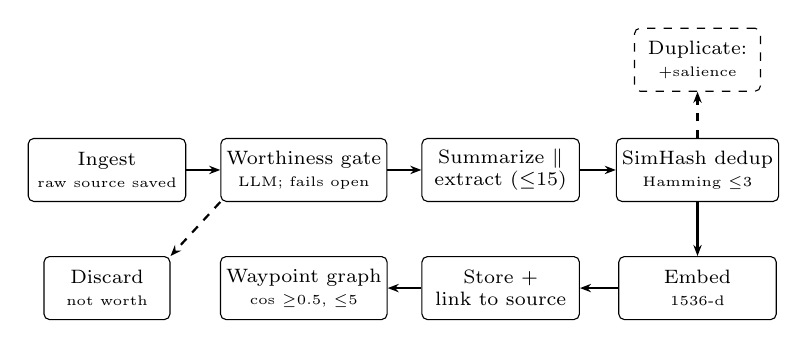
\begin{tikzpicture}
\node[box] (a) at (0,0) {Ingest\\{\tiny raw source saved}};
\node[box] (b) at (2.5,0) {Worthiness gate\\{\tiny LLM; fails open}};
\node[box] (c) at (5.0,0) {Summarize $\parallel$\\extract ($\le$15)};
\node[box] (d) at (7.5,0) {SimHash dedup\\{\tiny Hamming $\le$3}};
\node[box] (e) at (7.5,-1.5) {Embed\\{\tiny 1536-d}};
\node[box] (f) at (5.0,-1.5) {Store +\\link to source};
\node[box] (g) at (2.5,-1.5) {Waypoint graph\\{\tiny cos $\ge$0.5, $\le$5}};
\node[box,minimum width=1.6cm] (x) at (0,-1.5) {Discard\\{\tiny not worth}};
\node[box,minimum width=1.6cm,opt] (y) at (7.5,1.4) {Duplicate:\\{\tiny +salience}};
\draw[arr] (a) -- (b); \draw[arr] (b) -- (c); \draw[arr] (c) -- (d);
\draw[arr] (d) -- (e); \draw[arr] (e) -- (f); \draw[arr] (f) -- (g);
\draw[arr,opt] (b.south west) -- (x.north east);
\draw[arr,opt] (d.north) -- (y.south);
\end{tikzpicture}}
\caption{Ingestion pipeline. The gate defaults to ``worth remembering'' on LLM
timeout. Duplicates are not stored; they reinforce the existing memory's
salience. Waypoints are built asynchronously.}
\label{fig:pipeline}
\end{figure}

\subsection{Data Model}
Table~\ref{tab:schema} lists core entities. A \texttt{memory} carries content,
a SimHash, a cognitive \emph{sector} label (semantic, episodic, procedural,
emotional, reflective), a salience score, tags, and a 1536-d embedding, scoped
by \texttt{owner\_id}, \texttt{end\_user\_id}, \texttt{api\_key\_id} and
\texttt{project\_id}. \texttt{waypoints} form the memory graph;
\texttt{memory\_sources} records provenance.

\begin{table}[t]
\caption{Core data model (abridged).}
\label{tab:schema}
\centering
\footnotesize
\begin{tabular}{@{}ll@{}}
\toprule
Table & Purpose \\
\midrule
\texttt{users}, \texttt{api\_keys} & accounts, developer keys (bcrypt) \\
\texttt{end\_users} & inner tenant within an owner account \\
\texttt{sources} & raw content (JSONB), summary, vector \\
\texttt{memories} & atomic memories + 1536-d embedding \\
\texttt{waypoints} & weighted graph edges between memories \\
\texttt{memory\_sources} & N:N memory$\leftrightarrow$source provenance \\
\texttt{entities}, \texttt{memory\_entities} & extracted entities + links \\
\texttt{projects} & workspace grouping \\
\bottomrule
\end{tabular}
\end{table}

\subsection{Hybrid Retrieval Mechanism}
\label{sec:retrieval}
The sector taxonomy, waypoint graph and fused scoring follow the design of
OpenMemory~\cite{openmemory}; we adapted them to our pipeline and schema and
evaluate which components contribute. Given a query (Figure~\ref{fig:retrieval}): (1) intent phrases and stop words are
stripped; (2) the query sector is classified; (3) the query is embedded; (4)
pgvector returns the nearest $\min(2k,30)$ memories by cosine distance, where $k$
is the requested result count; (5) only if the mean candidate similarity is below
0.5 \emph{and} fewer than $k$ candidates were returned, the memory graph is
expanded via waypoints; (6) the candidate pool is re-scored with a fused score
\begin{equation}
\begin{split}
s = \operatorname{sigmoid}\big(&0.30\,\phi(\sigma) + 0.15\,o + 0.10\,w \\
 &+ 0.10\,r + 0.15\,t + 0.20\,c\big),
\end{split}
\end{equation}
where $\sigma$ is sector-adjusted cosine similarity,
$\phi(\sigma)=1-e^{-3\sigma}$ a boosting transform, $o$ lexical overlap with the
cleaned query, $w$ waypoint weight, $r$ recency, $t$ tag match, and $c$ a
coactivation term (Table~\ref{tab:weights}). The outer sigmoid is monotonic and
does not change the ranking.

Three properties bound what retrieval can claim. First, the fused score only
\emph{re-ranks} the pool returned by vector search, so it cannot surface a memory
that vector search missed. Second, because the pool holds $\min(2k,30)$ items,
the graph-expansion condition in step~(5) is false whenever a user has at least
$k$ memories, so waypoint expansion is effectively inactive for established
users; the waypoint graph serves primarily the visualization and provenance
features. Third, the coactivation term is implemented but the corresponding
recall counters are not persisted in the current schema, so $c=0$ in the
deployed system. Retrieved memories are reinforced asynchronously (salience and
last-seen time are updated, and co-recalled waypoints are strengthened); salience
itself is not an input to $s$, so reinforcement affects ranking only through
recency. For reproducible evaluation reinforcement is disabled, and two reduced
scoring modes are provided as ablation baselines (Section~\ref{sec:method}).

\begin{figure}[t]
\centering
\resizebox{\columnwidth}{!}{%
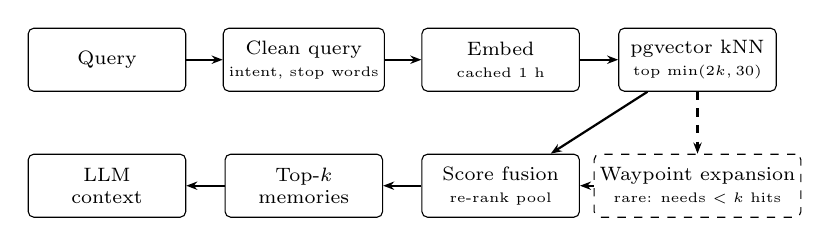
\begin{tikzpicture}
\node[box] (q) at (0,0) {Query};
\node[box] (c) at (2.5,0) {Clean query\\{\tiny intent, stop words}};
\node[box] (e) at (5.0,0) {Embed\\{\tiny cached 1 h}};
\node[box] (k) at (7.5,0) {pgvector kNN\\{\tiny top $\min(2k,30)$}};
\node[box,opt] (w) at (7.5,-1.6) {Waypoint expansion\\{\tiny rare: needs $<k$ hits}};
\node[box] (s) at (5.0,-1.6) {Score fusion\\{\tiny re-rank pool}};
\node[box] (t) at (2.5,-1.6) {Top-$k$\\memories};
\node[box] (l) at (0,-1.6) {LLM\\context};
\draw[arr] (q) -- (c); \draw[arr] (c) -- (e); \draw[arr] (e) -- (k);
\draw[arr] (k) -- (s);
\draw[arr,opt] (k) -- (w); \draw[arr,opt] (w) -- (s);
\draw[arr] (s) -- (t); \draw[arr] (t) -- (l);
\end{tikzpicture}}
\caption{Hybrid retrieval. Scoring re-ranks only the vector-search pool. Recency,
graph and coactivation signals are present in the code but not exercised in our
evaluation (Section~\ref{sec:retrieval}).}
\label{fig:retrieval}
\end{figure}

\begin{table}[t]
\caption{Hybrid scoring weights (production defaults). In the deployed schema
$c$ is always 0 and $w$ is non-zero only when graph expansion triggers.}
\label{tab:weights}
\centering
\footnotesize
\begin{tabular}{@{}lc|lc@{}}
\toprule
Signal & Weight & Signal & Weight \\
\midrule
Vector similarity $\phi(\sigma)$ & 0.30 & Recency $r$ & 0.10 \\
Lexical overlap $o$ & 0.15 & Tag match $t$ & 0.15 \\
Waypoint $w$ & 0.10 & Coactivation $c$ & 0.20 \\
\bottomrule
\end{tabular}
\end{table}

% ============================================================ 4 IMPLEMENTATION
\section{Implementation}\label{sec:impl}
\subsection{Technology Stack}
The backend is FastAPI (Python) with PostgreSQL and the pgvector extension;
embeddings and extraction use OpenAI models (\texttt{text-embedding-3-small};
\texttt{gpt-4o-mini}). Both dashboards are Next.js~14 + TypeScript + Tailwind
CSS with Firebase authentication. The API is deployed on Railway and the
dashboards on Vercel.

\subsection{Developer API and SDKs}
A stable \emph{Core API} (\texttt{POST /memories}, \texttt{GET /memories},
\texttt{POST /search}) is wrapped by evolvable \emph{Ingest} endpoints
(\texttt{/ingest/text|chat|document}) that perform LLM extraction, and a
\emph{Platform} API for keys and accounts. Developer keys are bcrypt-hashed with
a \texttt{um\_live\_} prefix. Two SDKs---\texttt{unimemory} on npm and
PyPI---wrap the Core API. A minimal integration is shown in
Listing~\ref{lst:sdk}.

\begin{lstlisting}[caption={JavaScript SDK integration.},label={lst:sdk}]
import UniMemory from 'unimemory';
const client = new UniMemory({ apiKey: process.env.UNIMEMORY_API_KEY });
await client.ingestText({
  content: "I'm vegetarian and allergic to peanuts",
  userId: "user123"
});
const hits = await client.search({ query: "any allergies?", userId: "user123" });
\end{lstlisting}

\subsection{Consumer Integration Layer}
The \emph{browser extension} (Chromium-based) captures chat content through
content scripts and a background service worker, authenticating with a consumer
session token; a keyboard-triggered popup surfaces stored sources on any page.
The \emph{MCP server} exposes memory to AI coding tools through tools for source
capture, memory search, memory-context retrieval and project status, so a fact
captured in one tool is retrievable in another. The \emph{consumer dashboard}
presents a memory timeline, an activity feed, semantic search, and a
Canvas-rendered \emph{memory graph} of projects, documents, memories and
entities. All clients share one backend and one store (Figure~\ref{fig:arch}).





\subsection{Deployment Status}
The API (Railway), both dashboards (Vercel), the Postgres/pgvector database
(Supabase) and both SDKs (\texttt{unimemory} on npm and PyPI) are deployed or
published. Source code is available at the repository linked on the title page.

% ============================================================ 5 METHODOLOGY
\section{Evaluation Methodology}\label{sec:method}
\subsection{Objectives}
We ask: (RQ1) does memory augmentation improve answer quality and cross-session
continuity over a stateless LLM? (RQ2) do \emph{extracted} memories retrieve
better, and more cheaply, than raw-chat RAG? (RQ3) does hybrid re-ranking
improve over lexical-only and pure-cosine scoring? (RQ4) what is the latency and deduplication
cost?

\subsection{Dataset}
We author a fictional persona (``Alex'') of ten short conversations across four
categories---preferences, projects, personal facts and events---each annotated
with ground-truth facts. Queries are split into a held-out \emph{test} set
(12 queries) and a \emph{dev} set (6 queries); scoring weights were never tuned
against the test set. Each query includes an exact phrasing and a paraphrase.
The corpus is synthetic and released with the harness for reproducibility.

\subsection{Protocol and Isolation}
All experiments run against a dedicated test user whose only data is the persona
corpus, so no real memories contaminate retrieval. Retrieval uses an eval-only
flag to disable asynchronous reinforcement, keeping repeated queries
deterministic; a second eval-only flag selects the scoring mode for the
ablation. Both flags are rejected by the server unless it is started in an
explicit evaluation mode, and neither changes production defaults. The dev set
is used for debugging and for the preliminary results reported here; the
held-out test set is run once, after the corpus is frozen.

\subsection{Conditions and Metrics}
\textbf{E1 (RQ1)} generates an answer with \texttt{gpt-4o-mini} with and without
the top-$k$ retrieved memories; answers are scored on a 0/1/2 rubric (0 generic
/ wrong, 1 partial, 2 correct and personalized) and also saved for manual
rating. \textbf{E2 (RQ2)} compares retrieval over extracted memories against a
raw-chat baseline that chunks and embeds the original conversations with the
\emph{same} embedding model; we report hit@$k$, MRR and context tokens injected.
\textbf{E3 (RQ3)} compares three scoring modes on exact and paraphrased queries
(hit@1/3/5, MRR): \texttt{cosine} (raw vector similarity), \texttt{lexical}
(boosted similarity + token overlap + tag match, no sector multiplier, waypoint
or recency) and \texttt{hybrid} (production scoring). All three re-rank the
\emph{same} candidate pool and use the \emph{same} cleaned query, so the cosine
baseline is slightly stronger than plain vector search on the raw query; this is
conservative for the hybrid scorer. Graph expansion, recency and coactivation are
not exercised by this corpus (all memories are created minutes apart, recall
counters are not persisted) and no result is attributed to them. \textbf{E4 (RQ4)} reports search
latency (mean/p50/p95 over 30 runs; latency against the Railway deployment
includes network time) and deduplication outcomes for exact, near- and
non-duplicate inputs. Relevance is keyword-grounded against the ground-truth
facts; E1 answers are additionally verified manually.

% ============================================================ 6 RESULTS
\section{Results}\label{sec:results}
\subsection{Preliminary Results (Development Set)}
The results below are a \emph{pilot} on the development query set: 6 queries
(12 instances counting exact and paraphrased phrasings) over 31 memories
extracted from the synthetic persona. They validate the method and the
evaluation harness; they are not the final evaluation, which runs once on the
held-out test set after the corpus is expanded. With this sample size, a
difference of a few instances is indicative, not statistically established.

\textbf{Memory on vs.\ off (E1).} Table~\ref{tab:e1} reports an
\emph{automated keyword rubric} (0--2), a sanity check rather than the blind
human-scored evaluation, which is pending. A stateless model cannot know
invented facts, so a score of 0.00 without memory is expected. With memory, one
personal-fact query (``Which college does Alex attend?'') scored 0: retrieval
ranked the correct memory (``final-year student at Somaiya'') first, but the
model did not map it to the question, a generation limitation rather than a
retrieval failure.

\begin{table}[t]
\caption{E1 (dev, automated keyword rubric, max 2): mean score.}
\label{tab:e1}
\centering\footnotesize
\begin{tabular}{@{}lcc@{}}
\toprule
Category (queries) & Memory off & Memory on \\
\midrule
Preferences (3)    & 0.00 & 2.00 \\
Projects (1)       & 0.00 & 2.00 \\
Personal facts (2) & 0.00 & 1.00 \\
Events (0)         & -- & -- \\
\midrule
\textbf{Overall (6)} & 0.00 & 1.67 \\
\bottomrule
\end{tabular}
\end{table}

\textbf{Structured memories vs.\ raw-chat RAG (E2).} Table~\ref{tab:e2} shows
that, on this small corpus, retrieval quality was identical: both conditions
placed a relevant item first for 5 of 6 queries and within the top three for
all 6. The measured difference is context size: the five retrieved extracted
memories averaged 55.2 tokens per query versus 86.8 for the five retrieved raw
message chunks. We therefore do not claim that structured memories retrieve
\emph{better}, only that they use less context here.

\begin{table}[t]
\caption{E2 (dev): retrieval quality (hits out of 6 queries) and mean tokens
injected per query (top-5 items).}
\label{tab:e2}
\centering\footnotesize
\begin{tabular}{@{}lccccc@{}}
\toprule
Condition & hit@1 & hit@3 & hit@5 & MRR & tokens \\
\midrule
Raw-chat RAG & 5/6 & 6/6 & 6/6 & 0.917 & 86.8 \\
Structured   & 5/6 & 6/6 & 6/6 & 0.917 & 55.2 \\
\bottomrule
\end{tabular}
\end{table}

\textbf{Scoring ablation (E3).} Table~\ref{tab:e3} compares the three scoring
modes. Hybrid and lexical scoring produced identical rankings on every query,
consistent with recency, graph and coactivation signals not contributing in this
setting; the gain over cosine is therefore attributable to token overlap, tag
matching and the similarity boost. Over all 12 instances hit@1 rose from 6/12
(cosine) to 9/12, and MRR from 0.715 to 0.861. The gap is concentrated in
paraphrased queries (hit@1 2/6 vs.\ 4/6). Because paraphrases were written by
the same author as the corpus, they may share vocabulary with the source facts,
which can favor lexical signals.

\begin{table}[t]
\caption{E3 (dev): scoring-mode ablation, hits out of 6 per phrasing.}
\label{tab:e3}
\centering\footnotesize
\begin{tabular}{@{}llcccc@{}}
\toprule
Phrasing & Mode & hit@1 & hit@3 & hit@5 & MRR \\
\midrule
Exact      & cosine  & 4/6 & 6/6 & 6/6 & 0.833 \\
Exact      & lexical & 5/6 & 6/6 & 6/6 & 0.917 \\
Exact      & hybrid  & 5/6 & 6/6 & 6/6 & 0.917 \\
Paraphrase & cosine  & 2/6 & 5/6 & 6/6 & 0.597 \\
Paraphrase & lexical & 4/6 & 6/6 & 6/6 & 0.805 \\
Paraphrase & hybrid  & 4/6 & 6/6 & 6/6 & 0.805 \\
\bottomrule
\end{tabular}
\end{table}

\subsection{Pending Measurements}
The following are not yet measured and are therefore not reported: final
held-out test-set results for E1--E3 (with blind human scoring for E1 and a
corpus expanded with distractor conversations); search latency, cold and warm;
and deduplication outcomes. They will be added to the final version.

% ============================================================ 7 CASE STUDY
\section{Cross-Tool Case Study}\label{sec:casestudy}
A qualitative demonstration of cross-tool continuity is planned: a preference
stated in a browser chat (captured by the extension) retrieved inside an AI IDE
through the MCP search tool without being restated. Annotated screenshots will
be added to the final version.

% ============================================================ 8 DISCUSSION
\section{Discussion and Limitations}\label{sec:discussion}
The pilot suggests that, over a small corpus, hybrid re-ranking improves
top-ranked precision relative to pure cosine similarity, mainly through lexical
signals, and that extracted memories can carry the same information in fewer
tokens than raw chat. It does not show that structured memories retrieve more
accurately, and it does not test the graph, recency or coactivation components.
Limitations: a single synthetic persona and very small query set, with corpus,
queries and paraphrases written by the same author; retrieval is already
near-saturated at hit@5 on 31 memories, so harder distractor corpora are
needed; a single LLM; hand-tuned (not learned) scoring weights; a worthiness
gate that fails open on timeout; keyword-grounded relevance; re-ranking limited
to the vector-search pool; coactivation inactive in the deployed schema; no
multi-user load testing; and no head-to-head benchmark against Mem0.

% ============================================================ 9 CONCLUSION
\section{Conclusion and Future Work}\label{sec:conclusion}
UniMemory is a deployed, reusable long-term memory layer with an end-to-end
pipeline, SDKs, an MCP server, a browser extension and two dashboards. A pilot
evaluation indicates that lexical re-ranking improves over pure vector
similarity and that extracted memories reduce injected context, pending
confirmation on a held-out test set. Future work includes a harder distractor
corpus, blind human scoring, latency and deduplication measurements, making the
coactivation signal functional by persisting recall statistics, evaluating graph
expansion, learned scoring weights, a Mem0 baseline on the same corpus, and
evaluation with real users.

\section*{Acknowledgment}
The authors thank their internal guide, Mr.\ Sunil Shelke, and their external
guide, Mr.\ Kunal Parekh (CPO, Osmos), for their guidance throughout this
project.

% ============================================================ REFERENCES
\bibliographystyle{IEEEtran}
\bibliography{references}

\end{document}
